% objectives.tex
\section{Research Objectives}
\label{objectives}
%
The objective of this project is to automatically map a given application requirements to physical hardware resources such that the application performance can be maintained in a highly consolidated environments. 

The virtualization layer will provide the framework to partition the available hardware resources and to isolate the performance interference between them\cite{}. 
The management layer will provide means to create a \emph{pool} of resources from cluster of heterogenous machines\cite{}, increasing the total amount of resources available for mapping. 
Live migration techniques\cite{} allow applications to be remaped based on the time varying demands and machine availbility. 
These mechanisms already exists in current virtulization infrastructure.
However, the mapping itself is still carried out manually decreasing the benefits of virtualization and explosing the system to the human error. 

To achieve our objective, the system must be aware of the workload changes, remap the resources and ensure that remaping satisfies the requirements all active applications.
A significant progress has already been made to migrate virtual machines to load balance CPU and memory resources\cite{}.
However, correct IO performance prediction is a much harder problem due to the statefulness of the storage systems\cite{}.
Another problem is that virtualization fails to isolate the performance interference of consolidated IO workloads as well as it isolates the CPU, memory and network resources. 
Last problem is lack of mapping between the application requirements and the virtualized resources. 
The actual application requirements are typically not specified interms of resource usage. 
Instead they are typically determined by the end user demand it must satisfy.   
A mechanism to monitor and model the application performance behavor is the last requirement of this project. 


\subsection{Intellectual Merit of the Proposed Work}
%
Describe the intellectual merit of the proposed work here.

\begin{figure}[h]
\centerline{\mbox{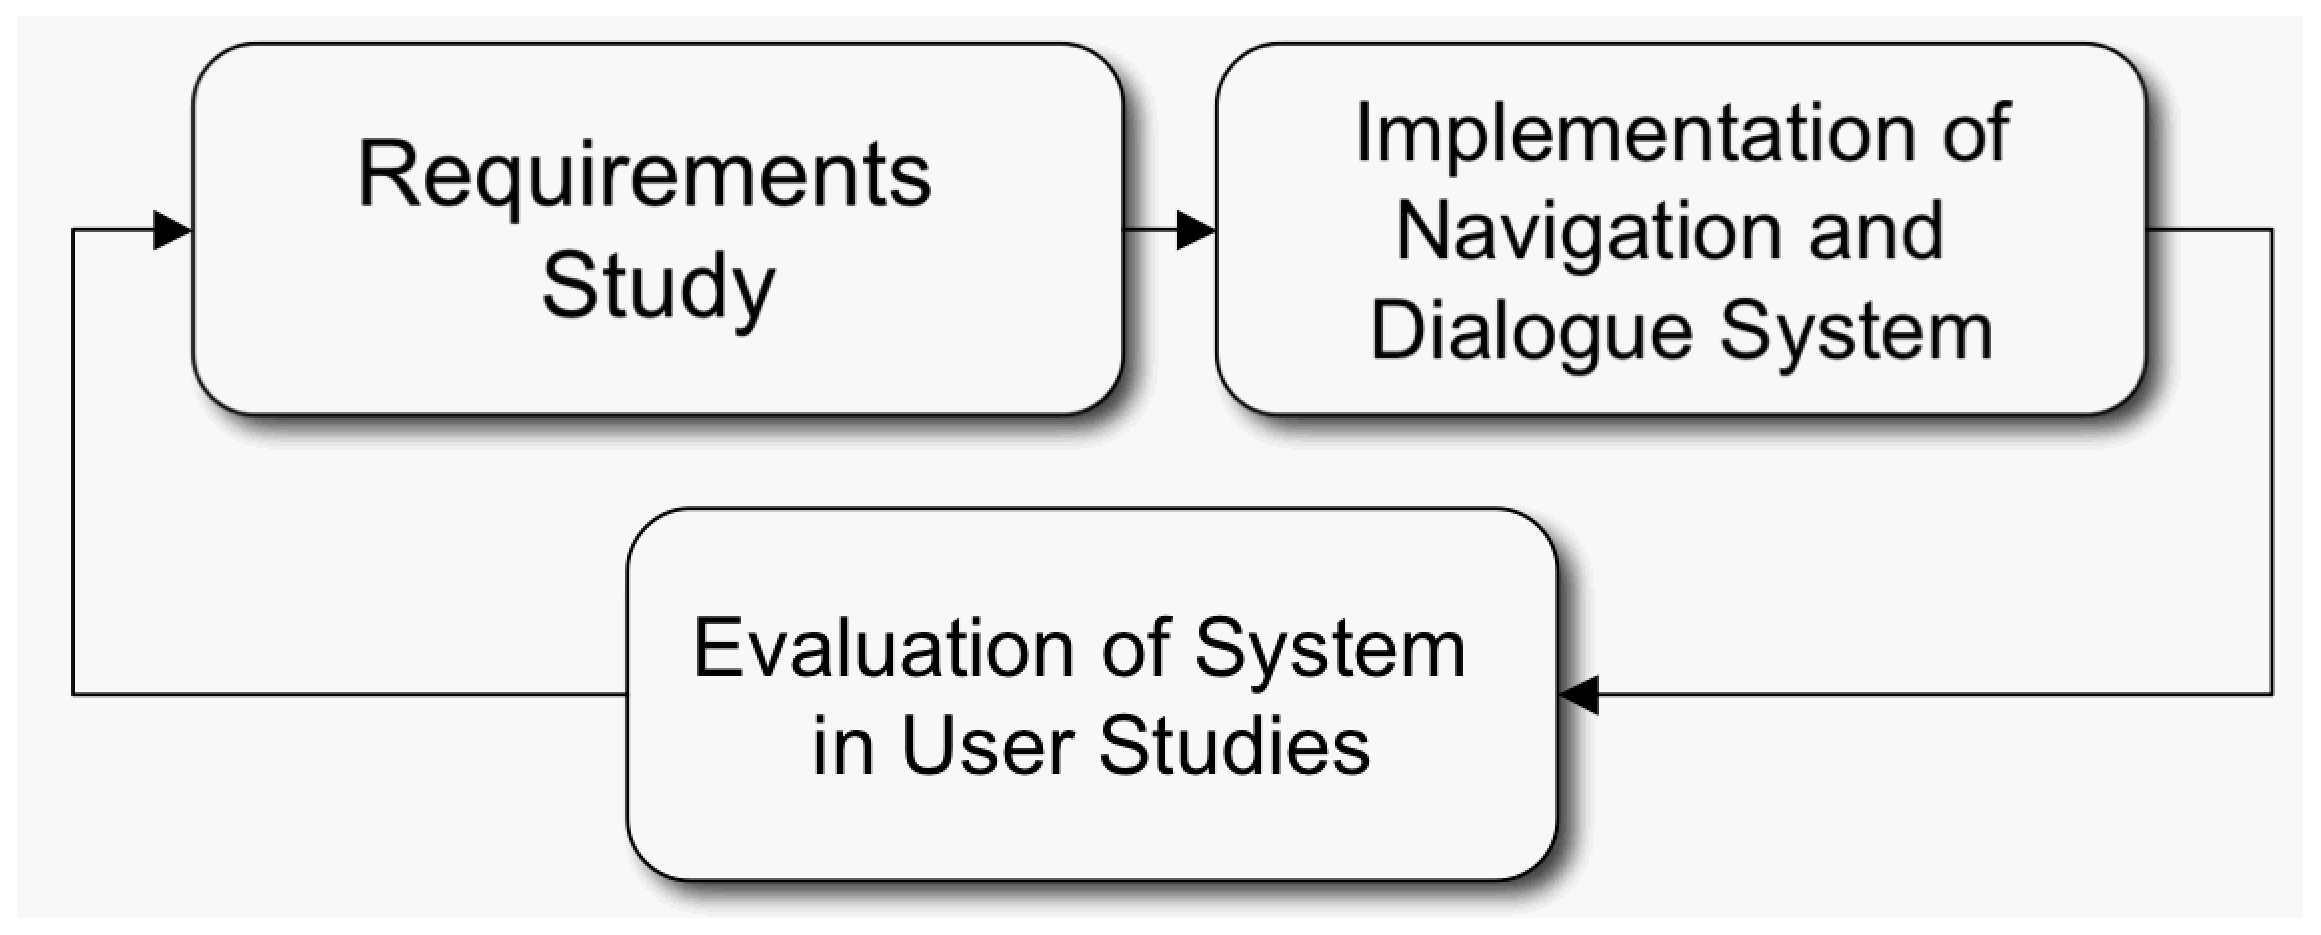
\includegraphics[width=3in]{cycle}}}
\caption{Our proposed research plan involves an iterated 
         cycle of design, implementation and user testing.}
\label{fig:cycle}
\end{figure}

Describe the intellectual merit of the proposed work here.

\subsection{Impact on VMware}
%
Describe the broader impact of the proposed work here.

Describe the broader impact of the proposed work here.
